% Provenance (never printed): see sources/outline_sources.md (Year 3:
% atmospheric dynamics: vorticity and potential vorticity, Rossby waves,
% baroclinic instability, the general circulation and the Hadley cell).
% Brief: sources/book5/BRIEFS.md, ch. 20. Curves from
% figdata/bachelor-3/rossby_waves.py, eady.py and held_hou.py. Exercise and
% problem values in the Book 5 scratch calculator calc/ch20.py. The waves,
% shears and parcels of the exercises and the problem are invented.
\chapter{Dinámica atmosférica}\label{ch:b3:atmospheric-dynamics}

En un mapa invernal de la troposfera superior, la corriente en chorro no rodea
el polo como un anillo liso. Serpentea en unas pocas ondas amplias que recorren
el hemisferio, con vaguadas que alcanzan los subtrópicos y dorsales hacia el
polo, y en superficie nacen depresiones que crecen durante unos pocos días y
mueren bajo ellas. Las ondas se desplazan lentamente, a veces en contra del viento que las
arrastra. Su número, su velocidad y el crecimiento de las borrascas bajo ellas
se derivan de una única magnitud conservada, la vorticidad del aire vista desde
el espacio, y de la energía almacenada en el contraste térmico entre los
trópicos y los polos.

\begin{recall}
La vorticidad y la circulación están en los libros de física. Las ondas de Rossby de la
troposfera superior, las vaguadas y las dorsales, el ciclón extratropical y el
principio de la predicción numérica del tiempo se describen en el volumen de segundo
año, en su capítulo sobre sistemas meteorológicos. Las células de Hadley, Ferrel y
polares, las corrientes en chorro, los vientos del oeste y el viento de momento angular de un anillo de
aire están en el volumen de primer año, en su capítulo sobre la circulación general de
la atmósfera, y el transporte de calor hacia los polos en su capítulo sobre
la radiación y el transporte de calor. El parámetro de Coriolis $f$, el plano $\beta$,
el radio de Rossby y el \omterm{thm:b3:gfd-foundations:thermal-wind}{viento térmico} están en
el capítulo~\ref{ch:b3:gfd-foundations}.
\end{recall}

\section{Vorticidad}\label{sec:b3:atmospheric-dynamics:vorticity}

La vorticidad de un fluido, el rotacional de su velocidad, es el doble de su
velocidad angular local. En la atmósfera a gran escala solo importa su
componente vertical, y a ella contribuye la rotación de la Tierra.

\begin{definition}[Vorticidad relativa, planetaria y absoluta]\label{def:b3:atmospheric-dynamics:vorticity-kinds}
Para una velocidad horizontal $(u, v)$, la \emph{vorticidad
relativa}\index{vorticidad relativa} es la componente vertical del rotacional
de la velocidad relativa al suelo, $\zeta = \partial v/\partial x -
\partial u/\partial y$, positiva para la rotación en sentido antihorario vista desde arriba.
La \emph{vorticidad planetaria}\index{vorticidad planetaria} es la componente vertical de la
vorticidad de la rotación terrestre, $2\Omega\sin\varphi =
f$. La \emph{vorticidad absoluta}\index{vorticidad absoluta} es su suma,
$\zeta + f$.
\end{definition}

En el hemisferio norte una depresión, donde el aire gira en sentido antihorario,
tiene $\zeta > 0$ y se llama ciclónica; un anticiclón tiene $\zeta < 0$. Un
viento de \qty{15}{m/s} que gira en un círculo de \qty{1000}{km} tiene $\zeta =
2V/R = \qty{3e-5}{s^{-1}}$ en rotación de sólido rígido, un tercio de $f$ a \ang{45}:
la parte planetaria suele ser la mayor.

\begin{theorem}[Ecuación de la vorticidad barotrópica]\label{thm:b3:atmospheric-dynamics:bve}
En un flujo bidimensional, no viscoso y sin divergencia horizontal sobre un
plano $\beta$, la \omterm{def:b3:atmospheric-dynamics:vorticity-kinds}{vorticidad absoluta} de cada partícula se conserva:
\[
\frac{\mathrm D(\zeta + f)}{\mathrm Dt} = 0 ,
\qquad\text{es decir}\qquad
\frac{\partial\zeta}{\partial t} + u\frac{\partial\zeta}{\partial x} + v\frac{\partial\zeta}{\partial y} + \beta v = 0 .
\]
Esta es la \emph{ecuación de la vorticidad barotrópica}\index{ecuación de la vorticidad barotrópica}.
\end{theorem}

\begin{proof}
Las ecuaciones horizontales del momento son $\mathrm Du/\mathrm Dt - fv =
-(1/\rho_0)\partial p/\partial x$ y $\mathrm Dv/\mathrm Dt + fu =
-(1/\rho_0)\partial p/\partial y$. Se deriva la segunda respecto de
$x$, la primera respecto de $y$, y se restan: la presión desaparece.
Con $\delta = \partial u/\partial x + \partial v/\partial y$, los
términos advectivos dan $\partial_x(u\,\partial_xv + v\,\partial_yv) -
\partial_y(u\,\partial_xu + v\,\partial_yu) = u\,\partial_x\zeta +
v\,\partial_y\zeta + \zeta\delta$, y los términos de Coriolis $f\delta + \beta
v$. Por tanto, $\mathrm D\zeta/\mathrm Dt + \beta v = -(\zeta + f)\,\delta$. Para
$\delta = 0$, y como $\mathrm Df/\mathrm Dt = \beta v$, $\mathrm D(\zeta +
f)/\mathrm Dt = 0$.
\end{proof}

La demostración da también la ley general, $\mathrm D(\zeta + f)/\mathrm Dt =
-(\zeta + f)\delta$: la convergencia acelera la rotación de una columna; la divergencia la
frena, como una patinadora que encoge o extiende los brazos. En una capa cuyo
espesor varía, la convergencia va ligada al estiramiento de la columna, y
la magnitud conservada pasa a ser una razón.

\begin{definition}[Vorticidad potencial]\label{def:b3:atmospheric-dynamics:pv}
La \emph{vorticidad potencial}\index{vorticidad potencial} de una columna de una
capa homogénea de espesor $h$ es $q = (\zeta + f)/h$. En un fluido continuamente
estratificado, la vorticidad potencial de Ertel es $q = (\vec\omega_a\cdot
\nabla\theta)/\rho$, siendo $\vec\omega_a$ el vector de \omterm{def:b3:atmospheric-dynamics:vorticity-kinds}{vorticidad absoluta} y
$\theta$ la temperatura potencial.
\end{definition}

\begin{theorem}[Conservación de la vorticidad potencial]\label{thm:b3:atmospheric-dynamics:pv}
En una capa homogénea, hidrostática y no viscosa de espesor variable $h$ cuya
velocidad horizontal no varía con la altura, $\mathrm Dq/\mathrm Dt = 0$
para $q = (\zeta + f)/h$.
\end{theorem}

\begin{proof}
A partir de la demostración anterior, $\mathrm D(\zeta + f)/\mathrm Dt = -(\zeta + f)\delta$.
La conservación de la masa en una columna de densidad uniforme da $\mathrm Dh/\mathrm
Dt = -h\delta$. Entonces $\mathrm Dq/\mathrm Dt = (1/h)\,\mathrm D(\zeta +
f)/\mathrm Dt - ((\zeta + f)/h^2)\,\mathrm Dh/\mathrm Dt = -(\zeta +
f)\delta/h + (\zeta + f)\delta/h = 0$.
\end{proof}

La forma de Ertel se conserva del mismo modo en un flujo adiabático y sin rozamiento
de un fluido estratificado, y la distancia entre dos superficies de $\theta$
constante hace el papel de $h$. Una columna de aire que atraviesa una
cordillera se comprime al ascender: su \omterm{def:b3:atmospheric-dynamics:vorticity-kinds}{vorticidad absoluta} disminuye, gira en
sentido anticiclónico sobre la cresta, y se estira y gira en sentido ciclónico
a sotavento. La conservación de la \omterm{def:b3:atmospheric-dynamics:vorticity-kinds}{vorticidad absoluta} o potencial es el
mecanismo restaurador de las ondas de la sección siguiente, como muestra la
figura de abajo.

\begin{omfigure}
\begin{tikzpicture}[>=stealth, font=\small, declare function={w(\x)=0.9*sin(\x r);}]
\draw[black!40, dashed] (0,0) -- (12.6,0) node[right, font=\scriptsize] {latitud $\varphi_0$};
\draw[thick, omDef, domain=0:12.566, samples=120] plot (\x, {w(\x)});
\foreach \x in {0.785, 2.356, 3.927, 5.498, 7.069, 8.639, 10.21, 11.78}
  \fill (\x, {w(\x)}) circle (0.06);
% crests: clockwise (anticyclonic), troughs: anticlockwise (cyclonic)
\foreach \x in {1.571, 7.854} {
  \draw[->, omThm, thick] (\x+0.45,{w(\x)+0.05}) arc (0:-300:0.45);
  \node[font=\scriptsize, omThm] at (\x,{w(\x)+0.75}) {$\zeta < 0$};}
\foreach \x in {4.712, 10.996} {
  \draw[->, omMeth, thick] (\x+0.45,{w(\x)-0.05}) arc (0:300:0.45);
  \node[font=\scriptsize, omMeth] at (\x,{w(\x)-0.75}) {$\zeta > 0$};}
\foreach \x in {3.1416, 9.4248} \draw[->, very thick] (\x,0.45) -- (\x,-0.45);
\foreach \x in {6.2832} \draw[->, very thick] (\x,-0.45) -- (\x,0.45);
\draw[->, thick] (8.4,-2.25) -- (6.4,-2.25) node[left, font=\scriptsize] {el patrón se desplaza hacia el O};
\draw[->] (0,-2.25) -- (1.4,-2.25) node[right, font=\scriptsize] {E};
\draw[->] (0,-2.25) -- (0,-1.65) node[above, font=\scriptsize] {N};
\end{tikzpicture}

\par\smallskip{\small Cómo se desplaza una onda de Rossby (esquema, hemisferio
norte). Una cadena de partículas en reposo a latitud $\varphi_0$ se
desplaza hasta formar una onda. Al conservarse $\zeta + f$, las partículas desplazadas hacia el norte, donde
$f$ es mayor, adquieren \omterm{def:b3:atmospheric-dynamics:vorticity-kinds}{vorticidad relativa} en sentido horario; las desplazadas al sur,
en sentido antihorario. Entre una cresta y la vaguada situada a su este, el flujo inducido
va hacia el sur, y entre una vaguada y la cresta situada a su este, hacia el norte (flechas
negras): la perturbación crece al oeste de cada cresta y todo el patrón
se desplaza hacia el O.}\label{fig:b3:atmospheric-dynamics:restoring}
\end{omfigure}

\section{Ondas de Rossby}\label{sec:b3:atmospheric-dynamics:rossby}

El volumen de segundo año describió las ondas de Rossby de la troposfera superior. La
\omterm{thm:b3:atmospheric-dynamics:bve}{ecuación de la vorticidad barotrópica} las explica. Se escribe el flujo como un
viento del oeste uniforme $U$ más una pequeña perturbación con función de corriente $\psi'$, de modo que
$u' = -\partial\psi'/\partial y$, $v' = \partial\psi'/\partial x$ y $\zeta'
= \nabla^2\psi'$.

\begin{theorem}[Dispersión de las ondas de Rossby]\label{thm:b3:atmospheric-dynamics:rossby}
Las pequeñas perturbaciones $\psi' \propto \mathrm e^{\mathrm i(kx + ly - \omega t)}$
de un viento del oeste uniforme $U$ en un plano $\beta$ cumplen la
\emph{relación de dispersión de las ondas de Rossby}\index{relación de dispersión de las ondas de Rossby}
\[
\omega = Uk - \frac{\beta k}{k^2 + l^2} .
\]
Su velocidad de fase hacia el este es $c = \omega/k = U - \beta/K^2$, con $K^2 =
k^2 + l^2$, y su velocidad de grupo hacia el este $c_g = \partial\omega/\partial
k = U + \beta(k^2 - l^2)/K^4$.
\end{theorem}

\begin{proof}
Linealizada en torno a $U$, la \omterm{thm:b3:atmospheric-dynamics:bve}{ecuación de la vorticidad barotrópica} queda
$(\partial_t + U\partial_x)\nabla^2\psi' + \beta\,\partial_x\psi' = 0$, despreciando los
productos de magnitudes pequeñas y que la $\zeta$ del flujo básico
sea nula. Para la onda plana, $\partial_t \to -\mathrm i\omega$,
$\partial_x \to \mathrm ik$ y $\nabla^2 \to -K^2$: $(-\mathrm i\omega +
\mathrm iUk)(-K^2) + \mathrm i\beta k = 0$, es decir $(\omega - Uk)K^2 =
-\beta k$. Derivando $\omega$ respecto de $k$ se obtiene $c_g = U -
\beta/K^2 + 2\beta k^2/K^4$, que es la forma enunciada.
\end{proof}

\begin{omfigure}
\begin{tikzpicture}
\begin{groupplot}[group style={group size=2 by 1, horizontal sep=1.7cm},
  width=0.48\linewidth, height=0.46\linewidth, tick label style={font=\scriptsize},
  label style={font=\small}, legend style={font=\scriptsize, draw=none, fill=none}]
\nextgroupplot[xlabel={número de onda zonal $n$}, ylabel={velocidad (\unit{m/s})},
  xmin=1, xmax=12, ymin=-40, ymax=60, legend pos=north east, legend cell align=left,
  title={\small \ang{45} N}]
% computed in figdata/bachelor-3/rossby_waves.py
\addplot[omThm, thick] table[x=n, y=c15] {figdata/out/bachelor-3-rossby_waves-disp.dat};
\addlegendentry{$c$, $U = 15$}
\addplot[omThm, thick, densely dashed] table[x=n, y=cg15] {figdata/out/bachelor-3-rossby_waves-disp.dat};
\addlegendentry{$c_g$, $U = 15$}
\addplot[omDef, thick] table[x=n, y=c0] {figdata/out/bachelor-3-rossby_waves-disp.dat};
\addlegendentry{$c$, $U = 0$}
\addplot[omDef, thick, densely dashed] table[x=n, y=cg0] {figdata/out/bachelor-3-rossby_waves-disp.dat};
\addlegendentry{$c_g$, $U = 0$}
\addplot[black!50, thin, domain=1:12, samples=2, forget plot] {0};
\nextgroupplot[xlabel={latitud (\unit{\degree} N)}, ylabel={número de onda estacionario $n_s$},
  xmin=20, xmax=75, ymin=0, ymax=9, legend pos=north east, legend cell align=left]
\addplot[omMeth, thick] table[x=lat, y=n10] {figdata/out/bachelor-3-rossby_waves-stat.dat};
\addplot[omDef, thick] table[x=lat, y=n15] {figdata/out/bachelor-3-rossby_waves-stat.dat};
\addplot[omThm, thick] table[x=lat, y=n20] {figdata/out/bachelor-3-rossby_waves-stat.dat};
\addplot[black, only marks, mark=*, mark size=1.1pt] table[x=lat, y=ns] {figdata/out/bachelor-3-rossby_waves-statobs.dat};
\legend{\qty{10}{m/s}, \qty{15}{m/s}, \qty{20}{m/s}, enero \qty{300}{hPa}}
\end{groupplot}
\end{tikzpicture}

\par\smallskip{\small A la izquierda, la velocidad de fase hacia el este $c$ (continua) y la
velocidad de grupo $c_g$ (a trazos) de las ondas de Rossby con $l = 0$ a \ang{45} N, frente al
número de ondas en torno al círculo de latitud, sin viento medio (azul)
y con un viento del oeste de \qty{15}{m/s} (rojo): las ondas largas se desplazan hacia el oeste, las cortas
son arrastradas hacia el este, y $c_g > c$. A la derecha, el número de onda estacionario para
vientos del oeste uniformes de 10, 15 y \qty{20}{m/s}, y para el viento medio zonal de enero
a \qty{300}{hPa} en cada latitud (puntos, NCEP--NCAR
Reanalysis~1, 1991--2020).}\label{fig:b3:atmospheric-dynamics:rossby}
\end{omfigure}
% ledger: data:b5-ncep-uwnd, geod5:grs80-defining, earth:Rmean

Respecto al aire, las ondas siempre se desplazan hacia el oeste, tanto más rápido
cuanto más largas son. Un viento del oeste arrastra hacia el este las ondas cortas; las largas
no puede arrastrar, y derivan hacia el oeste en contra del viento. Entre ambas, una
longitud de onda permanece inmóvil.

\begin{proposition}[Ondas de Rossby estacionarias]\label{prop:b3:atmospheric-dynamics:stationary}
En un viento del oeste $U > 0$, una onda sin estructura meridional ($l = 0$) es
estacionaria cuando su longitud de onda es la \emph{longitud de onda estacionaria de
Rossby}\index{longitud de onda estacionaria de Rossby} $\lambda_s =
2\pi\sqrt{U/\beta}$. Alrededor del círculo de latitud $\varphi$ esto equivale a un número entero de
ondas próximo a $n_s = \sqrt{2\Omega a\cos^3\varphi/U}$.
\end{proposition}

\begin{proof}
$c = 0$ cuando $k^2 = \beta/U$, luego $\lambda_s = 2\pi/k = 2\pi\sqrt{U/\beta}$.
La circunferencia tiene longitud $2\pi a\cos\varphi$, luego $n_s = a\cos\varphi\,k =
a\cos\varphi\sqrt{2\Omega\cos\varphi/(aU)} = \sqrt{2\Omega a\cos^3\varphi/U}$.
\end{proof}

A \ang{45} N, en un viento del oeste de \qty{15}{m/s}, con $\beta =
\qty{1.62e-11}{m^{-1}.s^{-1}}$, $\lambda_s = \qty{6050}{km}$ y $n_s =
4.7$: cuatro o cinco ondas alrededor del hemisferio. Con el viento medio zonal
de enero a \qty{300}{hPa}, de unos \qty{21}{m/s} a \ang{45} N, $n_s$ es
unas cuatro entre \ang{35} y \ang{55} N, y decrece hacia el polo. La velocidad de grupo
de una onda con $l = 0$ supera en $2\beta/k^2$ a su velocidad de fase: la energía avanza
por delante de la onda, de modo que una perturbación iniciada en un lugar genera nuevas vaguadas
y dorsales aguas abajo de ella, unos días después y a miles de kilómetros
al este, mientras que el patrón apenas se desplaza. Las cordilleras y los
contrastes de temperatura entre continentes y océanos fuerzan ondas estacionarias
de exactamente este tipo, a través del estiramiento y la compresión de
la \omterm{def:b3:atmospheric-dynamics:pv}{vorticidad potencial}.
% ledger: geod5:grs80-defining, earth:Rmean, data:b5-ncep-uwnd (values in figdata/bachelor-3/rossby_waves.py)


\section{Inestabilidad baroclínica}\label{sec:b3:atmospheric-dynamics:baroclinic}

Las ondas de la sección anterior son neutras: ni crecen ni decaen.
Las tormentas de las latitudes medias crecen y extraen su energía del
contraste de temperatura que expresa el \omterm{thm:b3:gfd-foundations:thermal-wind}{viento térmico}.

\begin{definition}[Energía potencial disponible]\label{def:b3:atmospheric-dynamics:ape}
La \emph{energía potencial disponible}\index{energía potencial disponible} de
un fluido estratificado es la diferencia entre su energía potencial total
(gravitatoria e interna) y la menor energía potencial total que puede
alcanzar mediante una redistribución adiabática de su masa, el estado en el que
las superficies de temperatura potencial constante, o de densidad potencial, son
horizontales.
\end{definition}

Un fluido con isentrópicas horizontales no tiene ninguna, por mucha energía potencial que
contenga; un fluido cuyas isentrópicas se inclinan, cálido y ligero de un lado, frío
y denso del otro, puede liberar algo dejándolas hundirse. Intercambiar
dos porciones de aire muestra cómo. Se toma una porción cálida baja en el lado ecuatorial y una
fría alta en el lado polar, ambas sobre la misma isentrópica en una atmósfera estable
cuyas isentrópicas ascienden hacia el polo. Intercambiarlas a lo largo de la
isentrópica no cambia nada. Intercambiarlas siguiendo una trayectoria menos empinada que la
isentrópica lleva la porción cálida hacia arriba y hacia el polo, a aire más frío que
ella misma, y la fría hacia abajo y hacia el ecuador, a aire más cálido: la cálida
asciende, la fría desciende, el centro de masas baja y se libera energía cinética
Las trayectorias dentro de esta cuña comprendida entre la horizontal y las
isentrópicas liberan energía; los \omterm{def:b3:atmospheric-dynamics:eddy}{remolinos} de latitudes medias son
intercambios que transportan calor hacia el polo y hacia arriba.

\begin{definition}[Inestabilidad baroclínica]\label{def:b3:atmospheric-dynamics:baroclinic-instability}
La \emph{inestabilidad baroclínica}\index{inestabilidad baroclínica} es la
inestabilidad de un flujo en rotación y estratificado en equilibrio de \omterm{thm:b3:gfd-foundations:thermal-wind}{viento térmico}, mediante el cual
las perturbaciones crecen al convertir la \omterm{def:b3:atmospheric-dynamics:ape}{energía potencial disponible} de las
isentrópicas inclinadas en su propia energía cinética.
\end{definition}

\begin{definition}[Modelo de Eady]\label{def:b3:atmospheric-dynamics:eady}
El \emph{modelo de Eady}\index{modelo de Eady} es un fluido de Boussinesq sobre un
plano $f$ comprendido entre dos superficies horizontales rígidas en $z = 0$ y $z = H$, con
\omterm{def:b3:gfd-foundations:buoyancy}{frecuencia de flotabilidad} $N$ uniforme y un viento del oeste que aumenta linealmente
con la altura, $U = \Lambda z$, en equilibrio de \omterm{thm:b3:gfd-foundations:thermal-wind}{viento térmico} con un
descenso uniforme de la temperatura hacia el polo; sus perturbaciones obedecen las
ecuaciones cuasigeostróficas.
\end{definition}

\begin{theorem}[Tasa de crecimiento de Eady]\label{thm:b3:atmospheric-dynamics:eady}
En el \omterm{def:b3:atmospheric-dynamics:eady}{modelo de Eady}, las perturbaciones $\propto \mathrm e^{\mathrm ik(x - ct)}$
con $\mu = kL_d$, $L_d = NH/f$, crecen exponencialmente cuando $\mu < \mu_c =
2.40$, a la tasa
\[
\sigma = \frac{f\Lambda}{N}\left[\left(\coth\frac{\mu}{2} - \frac{\mu}{2}\right)\left(\frac{\mu}{2} - \tanh\frac{\mu}{2}\right)\right]^{1/2} .
\]
La perturbación de crecimiento más rápido tiene $\mu = 1.61$, la longitud de onda $2\pi L_d/1.61
\approx 3.9\,L_d$, y crece a $\sigma_{\max} = 0.31\,f\Lambda/N$.
\end{theorem}
\admitted

La tasa de crecimiento depende solo de la cizalladura y de la estratificación, a través de
$f\Lambda/N$, y el tamaño preferido solo del radio de Rossby. Para la
media de enero a \ang{45} N el viento aumenta en \qty{17.2}{m/s} entre
\qty{850}{hPa} y \qty{250}{hPa}, a unos \qty{8.9}{km} de distancia en la
atmósfera estándar, una cizalladura de \qty{1.9e-3}{s^{-1}}; con la media
troposférica $N = \qty{0.0113}{s^{-1}}$ y $H = \qty{11}{km}$, $L_d =
\qty{1210}{km}$, la perturbación más rápida tiene una longitud de onda de \qty{4700}{km}
y crece por un factor $e$ en \num{2.1}~\text{días}. Las perturbaciones más cortas que
\qty{3200}{km} no crecen en absoluto. Estos son el tamaño y el tiempo de crecimiento de
las borrascas de un mapa del tiempo.
% ledger: data:b5-ncep-uwnd, nasa:grc-atmos (values in figdata/bachelor-3/eady.py)

\begin{omfigure}
\begin{minipage}[c]{0.52\linewidth}\centering
\begin{tikzpicture}
\begin{axis}[width=\linewidth, height=0.85\linewidth, xmin=2, xmax=16, ymin=0, ymax=0.55,
  xlabel={longitud de onda (\qty{1000}{km})}, ylabel={tasa de crecimiento (\unit{\text{día}^{-1}})},
  tick label style={font=\scriptsize}, label style={font=\small}]
% computed in figdata/bachelor-3/eady.py
\addplot[omThm, thick] table[x expr=\thisrow{lam}/1000, y=sday] {figdata/out/bachelor-3-eady-curve.dat};
\addplot[only marks, mark=*, mark size=1.6pt] coordinates {(4.721,0.4701)};
\node[font=\scriptsize, anchor=west] at (axis cs:5.0,0.49) {\qty{4700}{km}: amplificación $e$ en \qty{2.1}{d}};
\addplot[black!50, densely dashed] coordinates {(3.160,0) (3.160,0.55)};
\node[font=\scriptsize, anchor=west, black!60] at (axis cs:3.25,0.04) {corte};
\end{axis}
\end{tikzpicture}
\end{minipage}\hfill
\begin{minipage}[c]{0.44\linewidth}\centering
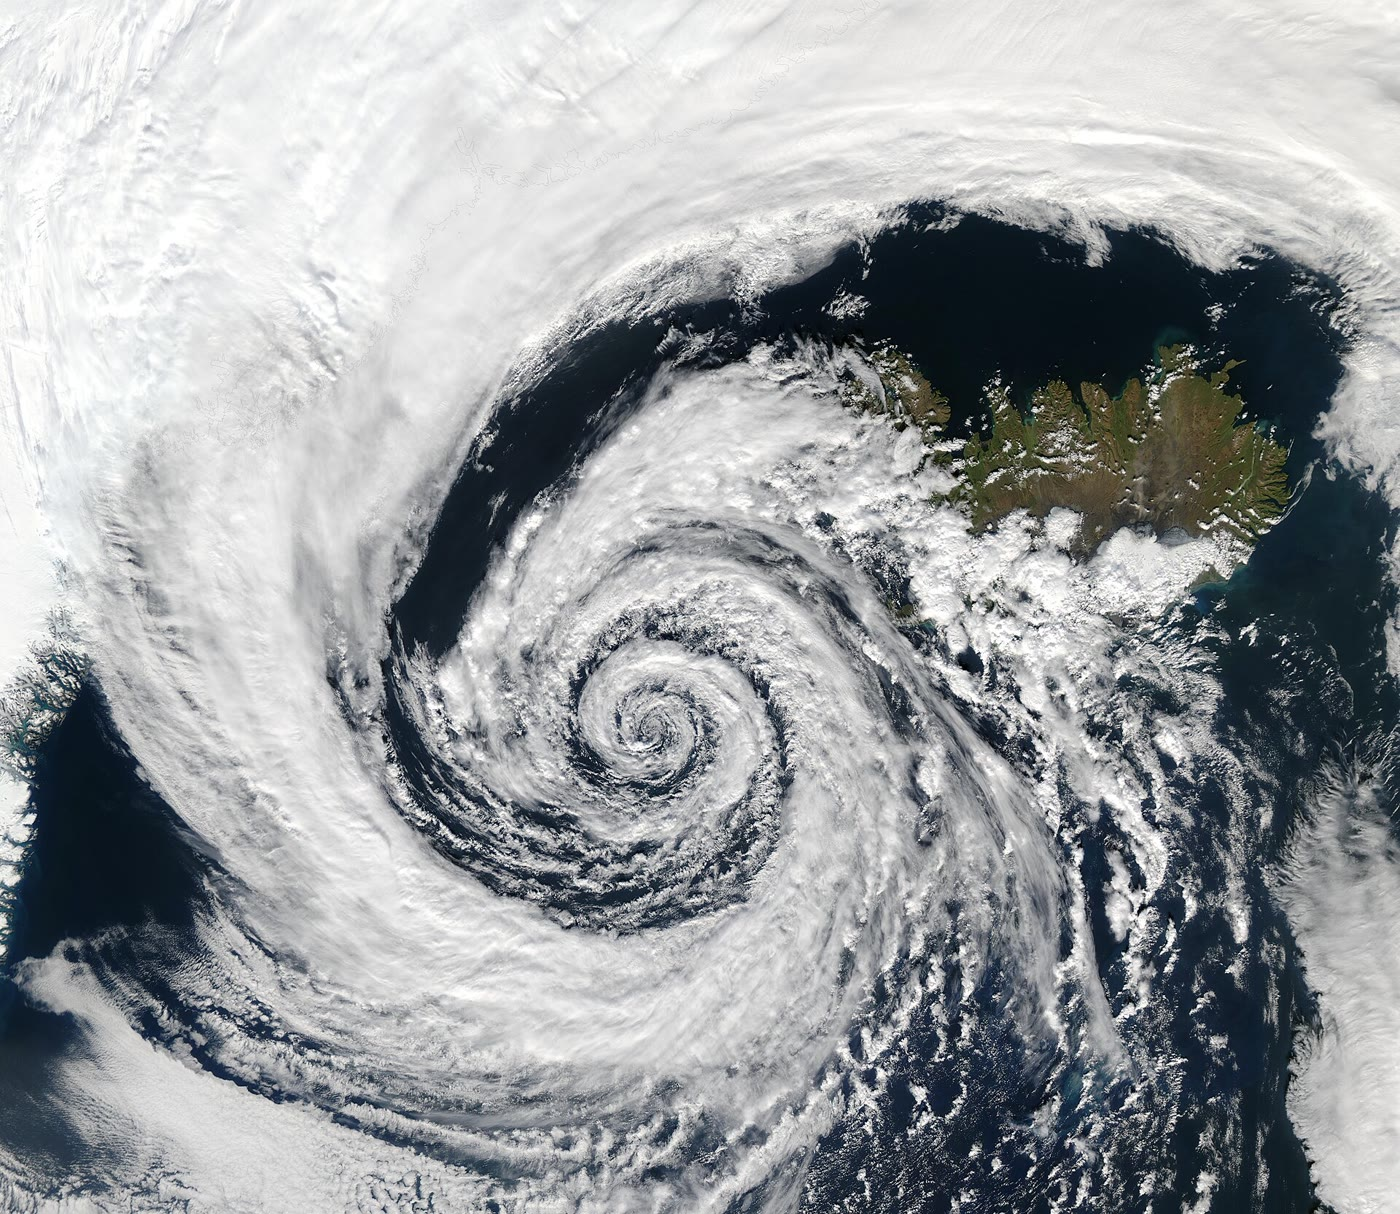
\includegraphics[width=\linewidth]{images/book5/b3-iceland-low.jpg}
\end{minipage}

\par\smallskip{\small A la izquierda, la tasa de crecimiento de Eady en función de la longitud de onda para la
cizalladura de la \omterm{def:b3:atmospheric-dynamics:eddy}{media zonal} de enero a \ang{45} N (NCEP--NCAR Reanalysis~1,
1991--2020), la estratificación troposférica media y $H = \qty{11}{km}$:
sin crecimiento por debajo de \qty{3200}{km}, y el crecimiento más rápido cerca de \qty{4700}{km}. A la derecha, una
borrasca en su fase madura frente a la costa suroeste de Islandia, el 4
de septiembre de 2003, con sus nubes enrolladas en espiral antihoraria alrededor de la
borrasca (NASA/GSFC, MODIS Rapid Response Team, dominio
público).}\label{fig:b3:atmospheric-dynamics:eady}
\end{omfigure}
% ledger: data:b5-ncep-uwnd, nasa:grc-atmos, photo:b3-iceland-low

El ciclón extratropical del volumen de segundo año es la cara superficial de una
onda baroclínica en crecimiento: su sector cálido transporta aire cálido hacia los polos y
hacia arriba, el aire frío que queda detrás desliza hacia el ecuador y hacia abajo, y la vaguada
en altura se inclina hacia el oeste al aumentar la altura, como exige la liberación de \omterm{def:b3:atmospheric-dynamics:ape}{energía potencial
disponible}.

\section{La circulación general}\label{sec:b3:atmospheric-dynamics:general-circulation}

La circulación general se describe promediando alrededor de los círculos de latitud,
y lo que el promedio omite es tan importante como lo que conserva.

\begin{definition}[Media zonal y remolinos]\label{def:b3:atmospheric-dynamics:eddy}
La \emph{media zonal}\index{media zonal} de una magnitud $A$ es su promedio
alrededor de un círculo de latitud a altura o presión fijas, $[A] =
(1/2\pi)\int_0^{2\pi} A\,\mathrm d\lambda$. La desviación $A^* = A - [A]$
es su parte de remolino; un \emph{remolino}\index{remolino (atmosférico)} de la
atmósfera es cualquier desviación del flujo respecto de su media zonal: ondas
viajeras, ondas estacionarias, ciclones y anticiclones.
\end{definition}

La \omterm{def:b3:atmospheric-dynamics:eddy}{media zonal} de un producto se descompone en dos: $[vT] = [v][T] + [v^*T^*]$. El
primer término es el transporte por la circulación meridiana media, las células
del volumen de primer año; el segundo, el transporte por los \omterm{def:b3:atmospheric-dynamics:eddy}{remolinos}. En las
latitudes medias el viento meridiano medio es débil y el término de \omterm{def:b3:atmospheric-dynamics:eddy}{remolinos}
domina: el aire que se desplaza hacia los polos es más cálido que el que se desplaza hacia el ecuador a la
misma latitud, como se muestra en la figura siguiente, y $[v^*T^*] > 0$. Los \omterm{def:b3:atmospheric-dynamics:eddy}{remolinos} también
transportan momento de los vientos del oeste, $[u^*v^*]$, desde los subtrópicos hacia las latitudes
de la corriente en chorro, por lo que la corriente en chorro y los vientos del oeste en superficie se
mantienen frente al rozamiento. La célula de Ferrel del volumen de primer año es la
circulación meridiana media que impone este transporte por \omterm{def:b3:atmospheric-dynamics:eddy}{remolinos}.

\begin{omfigure}
\begin{tikzpicture}[>=stealth, font=\small, declare function={s(\x)=0.9*sin(\x r); t(\x)=0.9*sin((\x+1.0) r);}]
\draw[thick, black, domain=0:12.566, samples=120] plot (\x, {s(\x)});
\draw[omThm, thick, densely dashed, domain=0:12.566, samples=120] plot (\x, {t(\x)-0.15});
\foreach \x in {0.3, 6.58} {\draw[->, omThm, very thick] (\x,-1.1) -- (\x,1.15)
  node[above, font=\scriptsize] {cálido};}
\foreach \x in {3.45, 9.73} {\draw[->, omDef, very thick] (\x,1.1) -- (\x,-1.15)
  node[below, font=\scriptsize] {frío};}
\node[font=\scriptsize, anchor=west, align=left] at (12.7,{s(12.566)}) {línea de\\ corriente};
\node[font=\scriptsize, anchor=west, omThm] at (12.7,{t(12.566)-0.15}) {isoterma};
\draw[->] (-1.6,-1.1) -- (-0.6,-1.1) node[below, font=\scriptsize] {este};
\draw[->] (-1.6,-1.1) -- (-1.6,-0.1) node[above, font=\scriptsize] {norte};
\node[font=\scriptsize] at (6.3,-1.95) {aire frío al norte, cálido al sur};
\end{tikzpicture}

\par\smallskip{\small Onda baroclínica en crecimiento en planta (esquema,
hemisferio norte, flujo del oeste). La isoterma (discontinua) va retrasada respecto a la
línea de corriente un cuarto de longitud de onda o menos, de modo que el aire que se desplaza al norte (flechas
rojas) es más cálido que el aire que se desplaza al sur a la misma latitud (azul):
la onda transporta calor hacia los polos, $[v^*T^*] >
0$.}\label{fig:b3:atmospheric-dynamics:heatflux}
\end{omfigure}

En los trópicos los \omterm{def:b3:atmospheric-dynamics:eddy}{remolinos} son débiles y la circulación media transporta calor
hacia los polos, la célula de Hadley. El volumen de primer año mostró que el aire que sale
del ecuador en reposo y conservando su momento angular soplaría a cientos de
metros por segundo a \ang{40}, y dejó abierta la cuestión de por qué la célula termina cerca de
\ang{30}. Un modelo sencillo responde.

\begin{definition}[Momento angular atmosférico; modelo de Held--Hou]\label{def:b3:atmospheric-dynamics:held-hou}
El \emph{momento angular atmosférico}\index{momento angular atmosférico}
por unidad de masa respecto al eje de la Tierra es $M = (\Omega a\cos\varphi +
u)\,a\cos\varphi$, para un viento hacia el este $u$ a la latitud $\varphi$. El
\emph{modelo de Held--Hou}\index{modelo de Held--Hou} de la célula de Hadley es una
circulación axisimétrica y estacionaria de una atmósfera seca de Boussinesq de profundidad
$H$, calentada por relajación hacia una temperatura potencial de equilibrio
radiativo $\theta_E/\theta_0 = 1 + \Delta/3 - \Delta\sin^2\varphi$; su
rama superior conserva $M$, su rama inferior tiene viento despreciable, y el
flujo se encuentra en equilibrio de \omterm{thm:b3:gfd-foundations:thermal-wind}{viento térmico}.
\end{definition}

\begin{theorem}[Extensión de la célula de Hadley]\label{thm:b3:atmospheric-dynamics:held-hou}
En el límite de ángulos pequeños, la célula de Held--Hou alcanza la latitud
\[
\varphi_H = \left(\frac{5\,gH\Delta}{3\,\Omega^2a^2}\right)^{1/2}
\]
en cada hemisferio, y el viento de su rama superior es $u_M = \Omega
a\varphi^2$.
\end{theorem}

\begin{proof}
Para $\varphi$ pequeño, $\cos\varphi \approx 1$ y el aire que sale del ecuador en
reposo con $M = \Omega a^2$ tiene $u_M = \Omega a(1 - \cos^2\varphi)/\cos\varphi
\approx \Omega a\varphi^2$. Con $f \approx 2\Omega\varphi$, $y = a\varphi$,
viento nulo en superficie y el \omterm{thm:b3:gfd-foundations:thermal-wind}{viento térmico} en su forma de Boussinesq sobre la
profundidad $H$, $2\Omega\varphi\,u_M/H = -(g/a\theta_0)\,\partial\theta_M/
\partial\varphi$, donde $\theta_M$ es la media vertical de $\theta$ en la
célula. Entonces $\partial(\theta_M/\theta_0)/\partial\varphi = -2\Omega^2a^2
\varphi^3/(gH)$ y $\theta_M/\theta_0 = A - K\varphi^4$, $K = \Omega^2a^2/
(2gH)$. Dentro de la célula la circulación mueve el calor, pero ni lo crea ni
lo destruye, de modo que la célula tiene la misma temperatura media que
el equilibrio radiativo: $\int_0^{\varphi_H}\theta_M\,\mathrm d\varphi = \int_0^{\varphi_H}
\theta_E\,\mathrm d\varphi$. En su borde la temperatura es continua:
$\theta_M(\varphi_H) = \theta_E(\varphi_H)$. Con $\theta_E/\theta_0 \approx
B - \Delta\varphi^2$, $B = 1 + \Delta/3$, la primera condición da $A - B =
K\varphi_H^4/5 - \Delta\varphi_H^2/3$, la segunda $A - B = K\varphi_H^4 -
\Delta\varphi_H^2$. Restando, $(4/5)K\varphi_H^4 = (2/3)\Delta
\varphi_H^2$, luego $\varphi_H^2 = 5\Delta/(6K) = 5gH\Delta/(3\Omega^2a^2)$.
\end{proof}

La célula termina donde la temperatura que impone la conservación del momento angular
se encuentra con el equilibrio radiativo; más allá, la atmósfera tendría que estar
más fría de lo que la radiación la hace. El modelo tiene dos parámetros que
no se observan directamente. Para $H = \qty{15}{km}$ y $\Delta$ entre $1/6$ y
$1/3$, elegido a modo de ilustración, $\varphi_H$ se sitúa entre \ang{25} y \ang{35}. Las
células observadas, leídas a partir del viento meridiano de \omterm{def:b3:atmospheric-dynamics:eddy}{media zonal}, terminan en
\ang{33.3} N y \ang{32.5} S en la media anual, y las células de invierno,
las más intensas, en \ang{30.8} N en diciembre--febrero y \ang{29.1} S en
junio--agosto. Lo importante es la escala: una célula que se ensancha con una
troposfera más profunda y un contraste de calentamiento más fuerte, y se estrecha en un
planeta de rotación más rápida. El viento superior del modelo, $u_M =
\qty{88}{m/s}$ en su borde para $\Delta = 1/6$, es el doble de la corriente en chorro observada:
los \omterm{def:b3:atmospheric-dynamics:eddy}{remolinos} se llevan el exceso.
% ledger: geod5:grs80-defining, earth:Rmean, data:b5-ncep-vwnd (values in figdata/bachelor-3/held_hou.py)

\begin{omfigure}
\begin{tikzpicture}
\begin{groupplot}[group style={group size=2 by 1, horizontal sep=1.7cm},
  width=0.48\linewidth, height=0.44\linewidth, tick label style={font=\scriptsize},
  label style={font=\small}, legend style={font=\scriptsize, draw=none, fill=none}]
\nextgroupplot[xlabel={latitud (\unit{\degree})}, ylabel={$100\,(\theta/\theta_0 - 1)$},
  xmin=0, xmax=60, ymin=-30, ymax=15, legend pos=south west, legend cell align=left,
  title={\small $\Delta = 1/3$, $H = \qty{15}{km}$}]
% computed in figdata/bachelor-3/held_hou.py
\addplot[omDef, thick] table[x=phi, y=thE] {figdata/out/bachelor-3-held_hou-theta-3.dat};
\addplot[omThm, thick, unbounded coords=jump] table[x=phi, y=thM] {figdata/out/bachelor-3-held_hou-theta-3.dat};
\addplot[black!50, densely dashed, forget plot] coordinates {(35.26,-30) (35.26,15)};
\node[font=\scriptsize, anchor=south west] at (axis cs:35.6,7) {$\varphi_H$};
\legend{$\theta_E$, $\theta_M$}
\nextgroupplot[xlabel={latitud (\unit{\degree})}, ylabel={$\psi$ en \qty{500}{hPa} ($10^{10}$\,\unit{kg/s})},
  xmin=-60, xmax=60, ymin=-25, ymax=25, xtick={-60,-30,0,30,60}, legend pos=south west,
  legend cell align=left]
\addplot[black!50, thin, domain=-60:60, samples=2, forget plot] {0};
\addplot[black, thick] table[x=lat, y=ann] {figdata/out/bachelor-3-held_hou-psi.dat};
\addplot[omDef, thick] table[x=lat, y=djf] {figdata/out/bachelor-3-held_hou-psi.dat};
\addplot[omThm, thick] table[x=lat, y=jja] {figdata/out/bachelor-3-held_hou-psi.dat};
\legend{año, DEF, JJA}
\end{groupplot}
\end{tikzpicture}

\par\smallskip{\small A la izquierda, la construcción de Held--Hou: la
temperatura de la célula que conserva el momento angular (rojo) alcanza el
equilibrio radiativo (azul) en $\varphi_H = \ang{35}$, con áreas iguales entre las
curvas dentro de la célula. A la derecha, la función de corriente másica meridional media en
\qty{500}{hPa} a partir del viento meridiano de \omterm{def:b3:atmospheric-dynamics:eddy}{media zonal} (NCEP--NCAR
Reanalysis~1, 1991--2020; positiva donde el aire por encima de \qty{500}{hPa}
se mueve hacia el norte): la intensa
célula del hemisferio de invierno abarca el ecuador, y las células terminan cerca de
\ang{30}.}\label{fig:b3:atmospheric-dynamics:held-hou}
\end{omfigure}
% ledger: data:b5-ncep-vwnd

\begin{history}[De las ondas largas al primer pronóstico calculado]
En 1939, C.-G.~Rossby y sus colaboradores, en el \emph{Journal of Marine
Research}, se propusieron interpretar varios fenómenos del tiempo aparentemente
independientes desde un único punto de vista. Motivados por configuraciones meteorológicas
que avanzan en sentido contrario al flujo dominante del oeste, Rossby formuló
una teoría linealizada en la que las perturbaciones de gran escala tienden a desplazarse hacia el oeste
y las de menor escala hacia el este respecto al viento: las ondas y el
plano $\beta$ de este capítulo. Once años después J.~G.~Charney,
R.~Fjørtoft y J.~von~Neumann integraron la \omterm{thm:b3:atmospheric-dynamics:bve}{ecuación de la vorticidad barotrópica}
de forma numérica en el ordenador electrónico ENIAC: cuatro pronósticos de 24~horas en
el nivel de \qty{500}{mb}, sobre una malla de \qty{736}{km}, de 8 grados de longitud
a \ang{45}. El cálculo de cada pronóstico tardó unas 24~horas; los autores
eran, como escribieron, apenas capaces de seguir el ritmo del tiempo.
\end{history}
% ledger: rossby39:paper, jmr20:commentary, charney50:eniac

\section{Ejercicios}

\begin{exercise}[$\star$]\label{exo:b3:atmospheric-dynamics:1}
(a)~Calcúlese la \omterm{def:b3:atmospheric-dynamics:vorticity-kinds}{vorticidad relativa} de un vórtice en rotación sólida que gira
una vez al día. (b)~Calcúlese la \omterm{def:b3:atmospheric-dynamics:vorticity-kinds}{vorticidad planetaria} a \ang{30} y \ang{60} N
($\Omega = \qty{7.292e-5}{rad/s}$) y compárense.
\end{exercise}

\begin{exercise}[$\star$]\label{exo:b3:atmospheric-dynamics:2}
Una parcela sin \omterm{def:b3:atmospheric-dynamics:vorticity-kinds}{vorticidad relativa} a \ang{30} N se desplaza hasta \ang{40} N en un
flujo sin divergencia. Calcúlese su \omterm{def:b3:atmospheric-dynamics:vorticity-kinds}{vorticidad relativa} en ese punto. ¿Es
ciclónica o anticiclónica?
\end{exercise}

\begin{exercise}[$\star$]\label{exo:b3:atmospheric-dynamics:3}
A \ang{45} N, sin viento medio, calcúlese la velocidad de fase de una onda de Rossby
de longitud de onda \qty{5000}{km} con $l = 0$. ¿En qué dirección se desplaza?
\end{exercise}

\begin{exercise}[$\star$]\label{exo:b3:atmospheric-dynamics:4}
A \ang{60} N, con viento del oeste de \qty{10}{m/s}, calcúlense $\beta$, la
longitud de onda estacionaria y el número de ondas estacionarias alrededor del
círculo de latitud ($a = \qty{6371}{km}$).
\end{exercise}

\begin{exercise}[$\star\star$]\label{exo:b3:atmospheric-dynamics:5}
Una columna de aire de \qty{10}{km} de profundidad, sin \omterm{def:b3:atmospheric-dynamics:vorticity-kinds}{vorticidad relativa} a \ang{45}
N, atraviesa una cordillera que la comprime hasta \qty{8}{km}, y después una cuenca
donde tiene \qty{12}{km} de profundidad. Suponiendo que se mantiene cerca de \ang{45} N, calcúlese su
\omterm{def:b3:atmospheric-dynamics:vorticity-kinds}{vorticidad relativa} sobre la cordillera y sobre la cuenca. ¿Dónde
tenderán a formarse las depresiones?
\end{exercise}

\begin{exercise}[$\star\star$]\label{exo:b3:atmospheric-dynamics:6}
Para la onda con cinco crestas alrededor del círculo de \ang{45} N ($l = 0$) en un
viento del oeste de \qty{15}{m/s}, calcúlense la velocidad de fase y la velocidad de grupo.
¿Cuánto tarda la energía de la onda en recorrer \qty{5000}{km} hacia el este, y
cuánto tarda el patrón?
\end{exercise}

\begin{exercise}[$\star\star$]\label{exo:b3:atmospheric-dynamics:7}
A \ang{45} N, con viento del oeste de \qty{15}{m/s}, una onda está confinada entre
latitudes tales que $l = \pi/(\qty{6000}{km})$. (a)~Calcúlense el número de onda
zonal estacionario y la longitud de onda. (b)~Demuéstrese que no existe ninguna onda estacionaria para
$l = \pi/(\qty{3000}{km})$.
\end{exercise}

\begin{exercise}[$\star\star$]\label{exo:b3:atmospheric-dynamics:8}
En un \omterm{def:b3:atmospheric-dynamics:eady}{modelo de Eady} a \ang{45} N, $\Lambda = \qty{2e-3}{s^{-1}}$, $N =
\qty{0.012}{s^{-1}}$ y $H = \qty{10}{km}$. Calcúlense $L_d$, la tasa de crecimiento
y el tiempo de $e$-folding de la perturbación de mayor crecimiento, y su
longitud de onda.
\end{exercise}

\begin{exercise}[$\star\star$]\label{exo:b3:atmospheric-dynamics:9}
A lo largo de un círculo de latitud, el viento meridiano del \omterm{def:b3:atmospheric-dynamics:eddy}{remolino} es $v^* = V\cos kx$ y la
temperatura del \omterm{def:b3:atmospheric-dynamics:eddy}{remolino} $T^* = T_0\cos(kx - \delta)$, con $V = \qty{10}{m/s}$ y
$T_0 = \qty{5}{K}$. Calcúlese $[v^*T^*]$ para $\delta = 0$, \ang{60} y
\ang{90}, y el flujo de calor correspondiente $\rho c_p[v^*T^*]$ por
\unit{kg/m^3} de aire ($c_p = \qty{1004}{J.kg^{-1}.K^{-1}}$). ¿Qué
disposición no transporta calor?
\end{exercise}

\begin{exercise}[$\star\star\star$]\label{exo:b3:atmospheric-dynamics:10}
Partiendo de la \omterm{thm:b3:atmospheric-dynamics:bve}{ecuación de la vorticidad barotrópica}, derívese la
\omterm{thm:b3:atmospheric-dynamics:rossby}{relación de dispersión de las ondas de Rossby} en un viento del oeste
uniforme, y demuéstrese que, respecto al aire, toda onda de Rossby se mueve hacia el oeste.
\end{exercise}

\begin{exercise}[$\star\star\star$]\label{exo:b3:atmospheric-dynamics:11}
En el \omterm{def:b3:atmospheric-dynamics:held-hou}{modelo de Held--Hou} tómese $H = \qty{12}{km}$ y $\Delta = 1/4$. Calcúlense
$\varphi_H$, el viento de ángulo pequeño $u_M$ en el borde y el viento exacto
de momento angular en ese punto, y compárense con el chorro subtropical de
\qty{44}{m/s} de la \omterm{def:b3:atmospheric-dynamics:eddy}{media zonal} de enero.
\end{exercise}

\begin{exercise}[$\star\star\star$]\label{exo:b3:atmospheric-dynamics:12}
Dos capas de aire difieren en temperatura potencial en \qty{10}{K} sobre
\qty{300}{K}; su interfaz asciende hacia el polo con pendiente $s$
a lo largo de una banda de \qty{4000}{km} de anchura, y $\rho = \qty{0.7}{kg/m^3}$. (a)~Demuéstrese
que dejar que la interfaz se aplane libera $\rho g' s^2L^2/24$ por unidad
de área, $g' = g\,\Delta\theta/\theta$. (b)~Calcúlese para $s = 10^{-3}$ y
$2\times10^{-3}$ y compárese con la energía cinética de un viento de \qty{15}{m/s}
a lo largo de \qty{10}{km} del mismo aire.
\end{exercise}
% ledger: geod5:grs80-defining, earth:Rmean, data:b5-ncep-uwnd

\section{Problema: la onda que permaneció quieta}

\begin{problem}[{Problema de fin de semana --- vorticidad, ondas de Rossby y el
crecimiento de una onda baroclínica a \ang{45} N}]
\label{pb:b3:atmospheric-dynamics:1}
Un flujo del oeste de \qty{15}{m/s} atraviesa las latitudes medias de un
continente ficticio, a lo largo de \ang{45} N. Tómense $\Omega =
\qty{7.292115e-5}{rad/s}$, $a = \qty{6371}{km}$ y $g = \qty{9.81}{m/s^2}$.
Todos los valores del flujo son ficticios.

\medskip\noindent\textbf{Parte I --- Una parcela desplazada.}
\begin{enumerate}
\item Una parcela sin \omterm{def:b3:atmospheric-dynamics:vorticity-kinds}{vorticidad relativa} a \ang{45} N se desplaza hasta
  \ang{50} N. Calcúlese $f$ en ambas latitudes y su \omterm{def:b3:atmospheric-dynamics:vorticity-kinds}{vorticidad relativa} a
  \ang{50} N, si el flujo no tiene divergencia.
\item Desplazándose a \qty{15}{m/s}, ¿con qué radio de curvatura gira
  (tómese $\zeta = -V/R$, todo debido a la curvatura)? ¿En qué sentido gira?
\item Si además su columna se reduce de \qty{10.0}{km} a \qty{9.5}{km} en el
  trayecto, ¿cuál es su \omterm{def:b3:atmospheric-dynamics:vorticity-kinds}{vorticidad relativa} a \ang{50} N?
\item Si, en cambio, se desplaza hasta \ang{40} N, sin divergencia, ¿qué \omterm{def:b3:atmospheric-dynamics:vorticity-kinds}{vorticidad relativa} adquiere?
  Explíquese por qué una parcela desplazada de su
  latitud oscila alrededor de ella.
\end{enumerate}

\medskip\noindent\textbf{Parte II --- Ondas viajeras.}
\begin{enumerate}[resume]
\item Calcúlense $\beta$ a \ang{45} N y la longitud del círculo de latitud.
\item Para $n = 3$ a 8 ondas alrededor del círculo ($l = 0$), calcúlense la
  longitud de onda, la velocidad de fase y la velocidad de grupo en el viento del oeste de
  \qty{15}{m/s}.
\item ¿Qué ondas se mueven hacia el oeste y cuáles hacia el este? ¿Cuántos días tarda la onda
  $n = 5$ en desplazarse \qty{1000}{km}?
\item Una dorsal sobre el oeste del continente se intensifica. ¿Dónde, y después de
  cuánto tiempo llegará el efecto de la onda $n = 6$ a \qty{5000}{km}
  aguas abajo?
\end{enumerate}

\medskip\noindent\textbf{Parte III --- La onda que permaneció quieta.}
\begin{enumerate}[resume]
\item Calcúlense la longitud de onda estacionaria y el número de onda estacionario a
  \ang{45} N.
\item Calcúlese el número de onda estacionario para vientos del oeste de 10 y
  \qty{20}{m/s}. ¿Qué ocurre con las ondas estacionarias cuando los vientos del oeste
  se intensifican en invierno?
\item Calcúlese el número de onda estacionario a \ang{35} N y \ang{55} N en el
  viento del oeste de \qty{15}{m/s}.
\item Las montañas del oeste del continente se elevan \qty{2}{km} en una
  troposfera de \qty{10}{km} de espesor. Calcúlese la \omterm{def:b3:atmospheric-dynamics:vorticity-kinds}{vorticidad relativa} de una columna
  que las atraviesa sin cambiar de latitud. ¿Por qué las montañas fuerzan
  ondas estacionarias?
\item ¿Por qué el patrón de ondas que forzan las montañas permanece quieto
  solo cuando su longitud de onda está cerca de $\lambda_s$?
\end{enumerate}

\medskip\noindent\textbf{Parte IV --- Crece una tormenta.}
\begin{enumerate}[resume]
\item El viento del oeste aumenta desde el suelo hasta \qty{10}{km} en
  \qty{25}{m/s}. Calcúlese la cizalladura $\Lambda$ y el gradiente de temperatura hacia el polo
  que implica el \omterm{thm:b3:gfd-foundations:thermal-wind}{viento térmico} a una temperatura media de
  \qty{250}{K}.
\item Con $N = \qty{0.011}{s^{-1}}$, calcúlese el número de Richardson
  $N^2/\Lambda^2$. ¿Es el flujo inestable frente a la turbulencia de cizalladura de pequeña escala?
\item Calcúlese el radio de Rossby $L_d$ para $H = \qty{10}{km}$.
\item Calcúlese la longitud de onda de la perturbación de Eady de mayor crecimiento y el
  número de estas ondas alrededor del círculo de latitud.
\item Calcúlese la longitud de onda más corta que crece.
\item Calcúlese la tasa de crecimiento $\sigma_{\max}$.
\item ¿En qué factor crece la perturbación en tres días?
\item Compárese la longitud de onda de la tormenta en crecimiento con la
  longitud de onda estacionaria de la Parte~III: ¿cuál es mayor, y qué implica eso para el
  movimiento de las tormentas respecto a las ondas estacionarias?
\item ¿Hacia qué lado se inclina con la altura la vaguada de la onda en crecimiento, y
  por qué debe hacerlo?
\item Indíquese el tiempo de $e$-folding de la perturbación de Eady de mayor crecimiento.
\end{enumerate}
\end{problem}
% ledger: geod5:grs80-defining, earth:Rmean
